\documentclass[a4paper,12pt]{article}
\usepackage[left=0.75in,right=0.75in,top=1.5in,bottom=1in,footskip=.25in]{geometry}
\usepackage{graphicx}
\usepackage[english]{babel}
\usepackage[utf8x]{inputenc}
\usepackage{url}
\usepackage{pgf-pie}


\newcommand{\Author}{Sanchit Kumar(40081187)}
\newcommand{\ProjectName}{Function 9: Power Function}
\newcommand{\Title}{}
\newcommand{\Course}{\textbf{SOEN-6011 \vspace{0.5cm} Software Engineering Processes}}
\newcommand{\ProfessorName}{Dr. PANKAJ KAMTHAN}

\begin{document}

%----------------------------------------------------------------------------------------
%	TITLE PAGE START
%----------------------------------------------------------------------------------------

\begin{titlepage}
\newcommand{\HRule}{\rule{\linewidth}{0.5mm}} %New command for thickness of line	


\centering
\textsc{\LARGE Concordia University} \\ [5mm] 
\includegraphics[scale=.1]{University_logo.jpg}\\[1cm] 
\textsc{\Large \Course} \\ [0.5cm]

%--------
%	TITLE
%--------
	
\HRule \\[0.4cm]
{ \huge \bfseries SCIENTIFIC CALCULATOR }\\[0.4cm] 
{\large \textbf{DELIVERABLE 3 (D3)} } \\ [0.2cm] 
{\large \textbf{Problem 5 \& 7} } \\ [0.2cm]
{\large \textbf{GitHub : \url{https://github.com/san089/SOEN-6011}}}	
\HRule \\[1.5cm]


%---------
%	TAIL SECTION
%---------
\vspace{7cm}
\Large \emph{\textbf{Author: \Author}}\\
{\large \today}\\[2cm]

\vfill
\end{titlepage}	



\newpage
%----------------------------------------------------------------------------------------
%	NEW PAGE START
%----------------------------------------------------------------------------------------
\begin{section}{Problem 7: Testing}

\subsection{Project Details}
\textbf{Below are the details about project.}
\renewcommand{\arraystretch}{1.5}
\begin{table}[htp]
	\centering
	\caption{Module 2 - $\tan(x)$} \vspace{0.5cm} \label{tab:definition_table} 
	\begin{tabular}{||c|c||}
		\hline \hline 
		\LARGE Project Name & \LARGE Scientific Calculator  \\ 
		\hline
		\LARGE Module Name & \LARGE $\tan(x)$  \\
		\hline
		\LARGE Developed By & \LARGE Anusha Keralapura Thandavamurthy \\
		\hline
		\LARGE Development End & \LARGE 29-July-2019 \\
		\hline  
		\LARGE Tested By & \LARGE Sanchit Kumar \\
		\hline 
		\LARGE Testing End & \LARGE 01-August-2019. \\
		\hline \hline
	\end{tabular}
\end{table}

\subsection{Testing Detailed Report}
\subsubsection{$\cos(x)$ Testing Reports}
\begin{itemize}
	
	\item \textbf{Test Case ID} \hspace{1.85cm} : TC1  \\
	\textbf{TYPE } \hspace{3.05cm}  : Functional\\
	\textbf{DESCRIPTION }\hspace{1.15cm} : $\cos(x)$ value test. \\
	\textbf{INPUT} \hspace{3.05cm} :  0.7853975 \\
	\textbf{EXPECTED RESULT} \hspace{0.01cm} : 0.7071072502792262 \\
	\textbf{ACTUAL RESULT} \hspace{0.6cm} : 0.7071072502792262 \\
	\textbf{TEST RESULT} \hspace{1.45cm} : PASS \\
	
	\item \textbf{Test Case ID} \hspace{1.85cm} : TC2  \\
	\textbf{TYPE } \hspace{3.05cm}  : Functional\\
	\textbf{DESCRIPTION }\hspace{1.15cm} : $\cos(x)$ value test. \\
	\textbf{INPUT} \hspace{3.05cm} :  0 \\
	\textbf{EXPECTED RESULT} \hspace{0.01cm} : 1 \\
	\textbf{ACTUAL RESULT} \hspace{0.6cm} : 1 \\
	\textbf{TEST RESULT} \hspace{1.45cm} : PASS \\	
	
	\item \textbf{Test Case ID} \hspace{1.85cm} : TC3  \\
	\textbf{TYPE } \hspace{3.05cm}  : Functional\\
	\textbf{DESCRIPTION }\hspace{1.15cm} : $\cos(x)$ value test. \\
	\textbf{INPUT} \hspace{3.05cm} :  3.14159 \\
	\textbf{EXPECTED RESULT} \hspace{0.01cm} : -1.0 \\
	\textbf{ACTUAL RESULT} \hspace{0.6cm} : -1.0000000035255 \\
	\textbf{TEST RESULT} \hspace{1.45cm} : FAIL \\
	
	
	\item \textbf{Test Case ID} \hspace{1.85cm} : TC4  \\
	\textbf{TYPE } \hspace{3.05cm}  : Functional\\
	\textbf{DESCRIPTION }\hspace{1.15cm} : $\cos(x)$ value test. \\
	\textbf{INPUT} \hspace{3.05cm} :  4.7123889 \\
	\textbf{EXPECTED RESULT} \hspace{0.01cm} : 0 \\
	\textbf{ACTUAL RESULT} \hspace{0.6cm} : -1.151329162868764E-5 \\
	\textbf{TEST RESULT} \hspace{1.45cm} : FAIL \\

%------------------------------------Sin Value Test--------------------------------------------
\subsubsection{$\sin(x)$ Testing Reports}
	
\item \textbf{Test Case ID} \hspace{1.85cm} : TC5  \\
\textbf{TYPE } \hspace{3.05cm}  : Functional\\
\textbf{DESCRIPTION }\hspace{1.15cm} : $\sin(x)$ value test. \\
\textbf{INPUT} \hspace{3.05cm} :  0.7853975 \\
\textbf{EXPECTED RESULT} \hspace{0.01cm} : 0.7071072502792262 \\
\textbf{ACTUAL RESULT} \hspace{0.6cm} : 0.7071072502792262 \\
\textbf{TEST RESULT} \hspace{1.45cm} : PASS \\

\item \textbf{Test Case ID} \hspace{1.85cm} : TC6  \\
\textbf{TYPE } \hspace{3.05cm}  : Functional\\
\textbf{DESCRIPTION }\hspace{1.15cm} : $\sin(x)$ value test. \\
\textbf{INPUT} \hspace{3.05cm} :  0 \\
\textbf{EXPECTED RESULT} \hspace{0.01cm} : 0 \\
\textbf{ACTUAL RESULT} \hspace{0.6cm} : 0 \\
\textbf{TEST RESULT} \hspace{1.45cm} : PASS \\	

\item \textbf{Test Case ID} \hspace{1.85cm} : TC7  \\
\textbf{TYPE } \hspace{3.05cm}  : Functional\\
\textbf{DESCRIPTION }\hspace{1.15cm} : $\sin(x)$ value test. \\
\textbf{INPUT} \hspace{3.05cm} :  3.14159 \\
\textbf{EXPECTED RESULT} \hspace{0.01cm} : 0 \\
\textbf{ACTUAL RESULT} \hspace{0.6cm} : 2.65306088421985E-6 \\
\textbf{TEST RESULT} \hspace{1.45cm} : FAIL \\


\item \textbf{Test Case ID} \hspace{1.85cm} : TC8  \\
\textbf{TYPE } \hspace{3.05cm}  : Functional\\
\textbf{DESCRIPTION }\hspace{1.15cm} : $\sin(x)$ value test. \\
\textbf{INPUT} \hspace{3.05cm} :  4.7123889 \\
\textbf{EXPECTED RESULT} \hspace{0.01cm} : -1 \\
\textbf{ACTUAL RESULT} \hspace{0.6cm} : -1.0000025759866482 \\
\textbf{TEST RESULT} \hspace{1.45cm} : FAIL \\


%------------------------------------Tan Value Test--------------------------------------------
\subsubsection{$\tan(x)$ Testing Reports}

\item \textbf{Test Case ID} \hspace{1.85cm} : TC9  \\
\textbf{TYPE } \hspace{3.05cm}  : Functional\\
\textbf{DESCRIPTION }\hspace{1.15cm} : $\tan(x)$ value test. \\
\textbf{INPUT} \hspace{3.05cm} :  39 \\
\textbf{EXPECTED RESULT} \hspace{0.01cm} : 0.809783081231065 \\
\textbf{ACTUAL RESULT} \hspace{0.6cm} : 0.809783081231065 \\
\textbf{TEST RESULT} \hspace{1.45cm} : PASS \\

\item \textbf{Test Case ID} \hspace{1.85cm} : TC10  \\
\textbf{TYPE } \hspace{3.05cm}  : Functional\\
\textbf{DESCRIPTION }\hspace{1.15cm} : $\tan(x)$ value test. \\
\textbf{INPUT} \hspace{3.05cm} :  0 \\
\textbf{EXPECTED RESULT} \hspace{0.01cm} : 0 \\
\textbf{ACTUAL RESULT} \hspace{0.6cm} : 0 \\
\textbf{TEST RESULT} \hspace{1.45cm} : PASS \\	

\item \textbf{Test Case ID} \hspace{1.85cm} : TC11 \\
\textbf{TYPE } \hspace{3.05cm}  : Functional\\
\textbf{DESCRIPTION }\hspace{1.15cm} : $\tan(x)$ value test. \\
\textbf{INPUT} \hspace{3.05cm} :  225 \\
\textbf{EXPECTED RESULT} \hspace{0.01cm} : 1 \\
\textbf{ACTUAL RESULT} \hspace{0.6cm} : 0.999993366047522 \\
\textbf{TEST RESULT} \hspace{1.45cm} : FAIL \\


\item \textbf{Test Case ID} \hspace{1.85cm} : TC12  \\
\textbf{TYPE } \hspace{3.05cm}  : Functional\\
\textbf{DESCRIPTION }\hspace{1.15cm} : $\tan(x)$ value test. \\
\textbf{INPUT} \hspace{3.05cm} :  315 \\
\textbf{EXPECTED RESULT} \hspace{0.01cm} : -1 \\
\textbf{ACTUAL RESULT} \hspace{0.6cm} : -1.0000092876074058 \\
\textbf{TEST RESULT} \hspace{1.45cm} : FAIL \\



%------------------------------------Tan Negative Value Test--------------------------------------------
\subsubsection{$\tan(x)$ Negative Values Testing Reports}

\item \textbf{Test Case ID} \hspace{1.85cm} : TC13  \\
\textbf{TYPE } \hspace{3.05cm}  : Functional\\
\textbf{DESCRIPTION }\hspace{1.15cm} : $\tan(x)$ negative value test. \\
\textbf{INPUT} \hspace{3.05cm} :  -64 \\
\textbf{EXPECTED RESULT} \hspace{0.01cm} : -2.0502989318619114  \\
\textbf{ACTUAL RESULT} \hspace{0.6cm} : -2.0502989318619114  \\
\textbf{TEST RESULT} \hspace{1.45cm} : PASS \\

\item \textbf{Test Case ID} \hspace{1.85cm} : TC14  \\
\textbf{TYPE } \hspace{3.05cm}  : Functional\\
\textbf{DESCRIPTION }\hspace{1.15cm} : $\tan(x)$ negative value test. \\
\textbf{INPUT} \hspace{3.05cm} :  -45 \\
\textbf{EXPECTED RESULT} \hspace{0.01cm} : -1 \\
\textbf{ACTUAL RESULT} \hspace{0.6cm} : -0.9999986732059835 \\
\textbf{TEST RESULT} \hspace{1.45cm} : FAIL \\	

\item \textbf{Test Case ID} \hspace{1.85cm} : TC15 \\
\textbf{TYPE } \hspace{3.05cm}  : Functional\\
\textbf{DESCRIPTION }\hspace{1.15cm} : $\tan(x)$ negative value test. \\
\textbf{INPUT} \hspace{3.05cm} :  -180 \\
\textbf{EXPECTED RESULT} \hspace{0.01cm} : 0 \\
\textbf{ACTUAL RESULT} \hspace{0.6cm} : 0 \\
\textbf{TEST RESULT} \hspace{1.45cm} : PASS \\



%------------------------------------Tan Decimal Value Test--------------------------------------------
\subsubsection{$\tan(x)$ Decimal Values Testing Reports}

\item \textbf{Test Case ID} \hspace{1.85cm} : TC16  \\
\textbf{TYPE } \hspace{3.05cm}  : Functional\\
\textbf{DESCRIPTION }\hspace{1.15cm} : $\tan(x)$ decimal value test. \\
\textbf{INPUT} \hspace{3.05cm} :  66.8 \\
\textbf{EXPECTED RESULT} \hspace{0.01cm} : 2.333168462359474 \\
\textbf{ACTUAL RESULT} \hspace{0.6cm} : 2.333168462359474  \\
\textbf{TEST RESULT} \hspace{1.45cm} : PASS \\

\item \textbf{Test Case ID} \hspace{1.85cm} : TC17  \\
\textbf{TYPE } \hspace{3.05cm}  : Functional\\
\textbf{DESCRIPTION }\hspace{1.15cm} : $\tan(x)$ decimal value test. \\
\textbf{INPUT} \hspace{3.05cm} :  1111111111111111111111.99999999999999999 \\
\textbf{EXPECTED RESULT} \hspace{0.01cm} : 0.62486935  \\
\textbf{ACTUAL RESULT} \hspace{0.6cm} : Program Not Responding \\
\textbf{TEST RESULT} \hspace{1.45cm} : FAIL \\	

\item \textbf{Test Case ID} \hspace{1.85cm} : TC18 \\
\textbf{TYPE } \hspace{3.05cm}  : Functional\\
\textbf{DESCRIPTION }\hspace{1.15cm} : $\tan(x)$ decimal value test. \\
\textbf{INPUT} \hspace{3.05cm} :  89.999999 \\
\textbf{EXPECTED RESULT} \hspace{0.01cm} : 57295779.814 \\
\textbf{ACTUAL RESULT} \hspace{0.6cm} : 743910.253181 \\
\textbf{TEST RESULT} \hspace{1.45cm} : FAIL \\

	
\end{itemize}


\subsection{Test Results Summary}
%----------------------------------------------------------------------
%               Test Case Impact
%----------------------------------------------------------------------

\begin{table}[htp]
	\centering
	\caption{Test Summary} \vspace{0.5cm} \label{tab:difficulty_table} 
	\begin{tabular}{||c|c|c||}
		\hline  \hline \textbf{Test Case ID} & \textbf{Status} & \textbf{Impact} \\
		\hline \hline
		TC1 & PASS & - \\ 
		\hline
		TC2 & PASS & - \\ 
		\hline
		TC3 & FAIL & Minor \\ 
		\hline
		TC4 & FAIL & Minor \\ 
		\hline
		TC5 & PASS & - \\ 
		\hline
		TC6 & PASS & - \\ 
		\hline
		TC7 & FAIL & Minor \\ 
		\hline
		TC8 & FAIL & Minor \\ 
		\hline
		TC9 & PASS & - \\ 
		\hline
		TC10 & PASS & - \\ 
		\hline
		TC11 & FAIL & Major \\ 
		\hline
		TC12 & FAIL & Major \\ 
		\hline
		TC13 & PASS & - \\ 
		\hline
		TC14 & FAIL & Major \\ 
		\hline
		TC15 & PASS & - \\ 
		\hline
		TC16 & PASS & - \\ 
		\hline
		TC17 & FAIL & Major \\ 
		\hline
		TC18 & FAIL & Major \\ 
		\hline	
	\end{tabular}
\end{table}


\subsection{Summary}
\centering
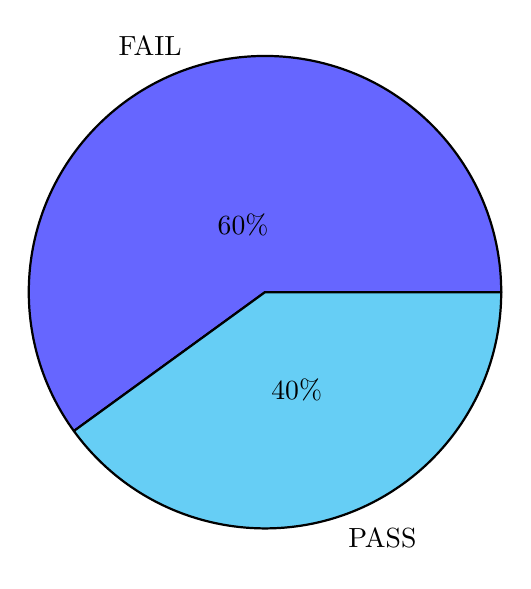
\begin{tikzpicture}
\pie{60/FAIL, 40/PASS}
\end{tikzpicture}


\end{section}





\end{document}